% !TEX options=--shell-escape
% https://github.com/SublimeText/LaTeXTools/issues/1082
%  _____ _             _    ______             __ _ __  
% |  ___(_)_ __   __ _| |  / /  _ \ _ __ __ _ / _| |\ \ 
% | |_  | | '_ \ / _` | | | || | | | '__/ _` | |_| __| |
% |  _| | | | | | (_| | | | || |_| | | | (_| |  _| |_| |
% |_|   |_|_| |_|\__,_|_| | ||____/|_|  \__,_|_|  \__| |
%                          \_\                      /_/ 
                   
% -------------------------------------------------------------------------
% https://www.kammerl.de/ascii/AsciiSignature.php - standard
% I've moved beyond justifying latex and am not just living in it.


% Use APA module
% Based on template from https://www.overleaf.com/latex/templates/your-apa6-style-manuscript/kngbbqpypjcq
\documentclass[a4paper,man,natbib,floatsintext]{apa6}
% Imports natbib
% Ref Sheet: https://gking.harvard.edu/files/natnotes2.pdf

% Packages
% Unicode in latex is a new, previously undiscovered circle of hell
\usepackage[english]{babel}
\usepackage[T1]{fontenc}
\usepackage[utf8x]{inputenc}
\usepackage{textcomp}
% /unicode
\usepackage{amsmath}
\usepackage{graphicx}
% set single spacing
\usepackage{setspace}
% glossary
\usepackage[acronym]{glossaries}
% fancy quotes
\usepackage{epigraph, varwidth}
% For formatting of potential bibliography
\usepackage{enumitem}
% html links
\usepackage{hyperref}
%\usepackage[colorinlistoftodos]{todonotes}
% Allow seperate footnotes
\usepackage{sepfootnotes}
% https://tex.stackexchange.com/questions/74170/have-new-line-between-paragraphs-no-indentation
\usepackage[parfill]{parskip}
% Diagrams!
\usepackage{svg}
\usepackage{graphicx}
\graphicspath{ {images/} }

% actually print contributors' name


% Trying to include graphics has been a JOURNEY
% Links used:
% aborted attempt to use svgs
% https://tex.stackexchange.com/questions/542766/inkscape-1-0-not-able-to-export-files-needed-for-svg-package
% https://tex.stackexchange.com/questions/2099/how-to-include-svg-diagrams-in-latex
% (updated comand line is: inkscape -D --export-latex  "EDEN_diagram.svg" --export-type="pdf" --export-filename="EDEN_diagram_svg-tex.pdf")
% https://www.overleaf.com/learn/latex/Inserting_Images
% convert EDEN_diagram.png -resize 50% EDEN_diagram.png


% This section was found in a stack overflow comment about making the epigraph length different and I include it here as an incantation against bad formatting
\renewcommand{\epigraphsize}{\small}
\setlength{\epigraphwidth}{0.6\textwidth}
\renewcommand{\textflush}{flushright}
\renewcommand{\sourceflush}{flushright}
% A useful addition
\newcommand{\epitextfont}{\itshape}
\newcommand{\episourcefont}{\scshape}

\makeatletter
\newsavebox{\epi@textbox}
\newsavebox{\epi@sourcebox}
\newlength\epi@finalwidth
\renewcommand{\epigraph}[2]{%
  \vspace{\beforeepigraphskip}
  {\epigraphsize\begin{\epigraphflush}
   \epi@finalwidth=\z@
   \sbox\epi@textbox{%
     \varwidth{\epigraphwidth}
     \begin{\textflush}\epitextfont#1\end{\textflush}
     \endvarwidth
   }%
   \epi@finalwidth=\wd\epi@textbox
   \sbox\epi@sourcebox{%
     \varwidth{\epigraphwidth}
     \begin{\sourceflush}\episourcefont#2\end{\sourceflush}%
     \endvarwidth
   }%
   \ifdim\wd\epi@sourcebox>\epi@finalwidth 
     \epi@finalwidth=\wd\epi@sourcebox
   \fi
   \leavevmode\vbox{
     \hb@xt@\epi@finalwidth{\hfil\box\epi@textbox}
     \vskip1.75ex
     \hrule height \epigraphrule
     \vskip.75ex
     \hb@xt@\epi@finalwidth{\hfil\box\epi@sourcebox}
   }%
   \end{\epigraphflush}
   \vspace{\afterepigraphskip}}}
\makeatother
% End epigraph modifications

\makenoidxglossaries
% These used to be in a seperate file, but I want them in here because it will let me cite things from the bibliography in them

%   _____ _                                
%  / ____| |                               
% | |  __| | ___  ___ ___  __ _ _ __ _   _ 
% | | |_ | |/ _ \/ __/ __|/ _` | '__| | | |
% | |__| | | (_) \__ \__ \ (_| | |  | |_| |
%  \_____|_|\___/|___/___/\__,_|_|   \__, |
%                                     __/ |
%                                    |___/ 


\newacronym{foss}{FOSS}{Free Open Source Software}
\newacronym{sts}{STS}{Science, Technology \& Society}
\newacronym{ict}{ICT}{Information and Communications Technology}
\newacronym{eden}{EDEN}{Emergency Development ENvironment}
\newacronym{ict4d}{ICT4D}{Information and Communication Technologies for Development}


\newglossaryentry{ICT}
{
    name=Information and communications technology,
    description={Information and communications technology: A term for the mix of physical devices and software that mix analog and digital techniques to allow communication, recall and storage of data.}
}
 
\newglossaryentry{FOSS}
{
    name=Free Open Source Software,
    description={Free Open Source Software: A method of developing software that does not charge for use of the software. The software's source code is also freely distributed, allowing users to modify their copy of the software or suggest changes to the organization developing it.}
}

\newglossaryentry{python}
{
    name=python,
    description={Python is an open source, interpreted, high-level, general-purpose programming language. It was initially released in the early 1990s, but has been continuously updated since then. Python 2 was the standard from 2000 to 2008, but in 2008 Python 3 was released with backwards-incompatible changes. This split the Python community, leading to Python 2 and Python 3 having slightly different versions of tools available. Python 2 continued to receive support and updates until 2020, when official support for Python ended (Wikipedia contributors, 2020). The open source nature of Python means that it is likely that Python 2 will continue to be updated by users after official support ends. }
}

\newglossaryentry{OpenStreetMap}
{
    name=OpenStreetMap,
    description={An open community of volunteers that maintain data about roads, trails, cafés, railway stations, and much more, all over the world.}
}
\newglossaryentry{web framework}
{
    name=web framework,
    description={A heterogeneous set of software that allow a programmer to efficiently write and manage providing a service over the Internet. This could be a website or a mobile app (often it is both) or a go-between for other services. Examples include web2py and Django in Python or Phoenix in Elixir.}
}

\newglossaryentry{PostgreSQL}
{
   name=PostgreSQL,
   description={PostgreSQL is a powerful, open source object-relational database system with over 30 years of active development that has earned it a strong reputation for reliability, feature robustness, and performance.}
   % https://www.postgresql.org/
}

% https://en.wikipedia.org/wiki/MySQL
%  MySQL is a component of the LAMP web application software stack (and others), which is an acronym for Linux, Apache, MySQL, Perl/PHP/Python. MySQL is used by many database-driven web applications, including Drupal, Joomla, phpBB, and WordPress
\newglossaryentry{MySQL}
{
   name=MySQL,
   description={MySQL is an open-source relational database management system (RDBMS). Its name is a combination of "My", the name of co-founder Michael Widenius's daughter, and "SQL", the abbreviation for Structured Query Language}
}

% http://eden.sahanafoundation.org/wiki/WikiStart#WhatisSahanaEden
\newglossaryentry{EDEN}
{
   name=EDEN,
   description={The Emergency Development ENvironment, developed by the Sahana Foundation, is an Open Source Humanitarian Platform which can be used to provide solutions for Disaster Management, Development, and Environmental Management sectors}
}

\newglossaryentry{ICT4D}
{
   name=Information and Communication Technologies for Development,
   description={The movement to use digital technologies to serve the needs of the underprivileged and those living in the developing world. Criticized for being directed more at the developed worlds' love of technology than the actual needs of those it purports to serve. Also called digital humanitarianism}
}

\newglossaryentry{capta}
{
   name=capta,
   description={If data is every piece of information about an entity, capta are the semantically meaningfull elements within that data (Kitchin \& Dodge, 2011). The data of DNA is the entire sequence and the capta would be (we think) the genes that encode for particular traits and proteins}
}

\newglossaryentry{srcd}
{
   name=source code,
   description={Human recognizable language, generally written in primaraly latin text in sets of files. Examples include C, Python (the language of EDEN), LaTeX (the language this paper is assembled by).}
}

\newglossaryentry{mscd}
{
   name=machine code,
   description={A language understood by a particular kind of computer chip. Can be generally understood as a list of specific instructions to the computer chip to do digital operations. I.e. add two numbers, load a value into memory, write a value to disk or send a value over the internet. Common machine languages would be x86 (most laptops and desktops) and ARM (most phones).}
}

\newglossaryentry{sp}
{
    name=software project,
    description={Drawing from \citet{Mackenzie2006-hb}, this is the total social, material and organizational structure associated with the production, distribtuon and use of a particular piece of software. This includes the people who work directly on the source code of any \gls{sa} associated with the project as well as anyone who is part of the organization that manages, funds and directs the development of the software. It may also involve people who are not employed by the formal owner of the software project (this is especially true for open source developers). Any \glspl{sa} assembled by members of the project who are acting as members (and not on their own) are also part of the project. \glspl{sa} assembled using source code from the project are not part of the project per-se, but the software project bears some measure of responsibility for how those \glspl{sa} function and act in the world.}
}

\newglossaryentry{sa}
{
    name=software artifact,
    description={An entity of uncertain composition that behaves, for common users (as opposed to technical staff) as a single entity. A software-artifact could be a single binary with all its functionality provided by machine code included in that single location in memory. It could also be a binary that makes calls to various libraries. In the case of EDEN, it's an expensive set of Python files - some of which are human readable and some of which have been modified to make them faster to read. In this case a separate program, the Python binary itself, reads and executes the EDEN program. Even though EDEN is many separate files and contains no machine code, it is properly considered a software-artifact because users interact with it as a single entity.  Software-artifacts are produced periodically by software projects, but are not themselves entirely "software." The idea of software must be large enough to allow multiple software-artifacts to exist within the same project: the current version of your phone OS and the next version, the Facebook app on your phone and the web server that tells it what has happened. Nevertheless, when we are using "software" we are always directly interacting with one or more software-artifact(s). They are the material reality of software projects.}
}

\newglossaryentry{webframework}
{
  name=Web Framework,
  description={A library (or set of libraries) that handles translation from and to the language of HTTP and other web technologies. The library of functionality they provide can range from wrapping basic text in a format a web browser will understand to providing functionality that allows users to log in, receive real-time messages and interact with the same web site from multiple clients simultaneously (Statz, 2010). Each Web framework also has its own philosophy about what information the developer is expected to provide and how much the developer needs to set. Some frameworks attempt to provide everything that is required to build almost any website, while others focus on providing a core of functionality and may not include support for connecting to a database or managing logins. Generally, any web framework may be used to make any website, but framework selection will dramatically change the experience of the software engineers developing that web site.}
}

\newglossaryentry{vm}
{
  name=Virtual Machine,
  description={A family of packaging techniques that allow packaging and distribution of an entire computing environment (operating system, libraries, programs) in a single digital object. This allows one physical computer to run several independent "machines" simultaneously. When a virtual machine is started, it the hardware it sees is virtual hardware simulated by the program "hosting" the virtual machine. The hosting program then translates requests to that virtual hardware into requests to the real hardware and relays the responses. Running a program in a virtual machine is slightly less efficient than running it on real hardware, but this cost is often less than the cost of manually arranging non-virtual installs on real machines.}
}

\newglossaryentry{sf}
{
  name=Sahana Foundation,
  description={The nonprofit that manages the EDEN project. Based in Los Angeles with an international scope and focuses on supporting communities in disaster preparedness and response through information technology.}
}

\newglossaryentry{w2p}
{
  name=Web2Py,
  description={An open source web framework for Python 2.7 and 3+.}
}

\newglossaryentry{cmp}
{
  name=Composite,
  description={A \citet{Latour1999-ui}ian black box whose functionality cannot be reduced to a blackbox containing other blackboxes. Instead, a composite is a network of blackboxes are heterogeneously linked. In addition, where the contents of a blackbox become socially visible when the blackbox stops working, composites can totally fail and remain opaque.}
}


% \newglossaryentry{}
% {
%    name=,
%    description={}
% }

%      _______ _                                
%     / / ____| |                               
%    / / |  __| | ___  ___ ___  __ _ _ __ _   _ 
%   / /| | |_ | |/ _ \/ __/ __|/ _` | '__| | | |
%  / / | |__| | | (_) \__ \__ \ (_| | |  | |_| |
% /_/   \_____|_|\___/|___/___/\__,_|_|   \__, |
%                                          __/ |
%                                         |___/ 

\singlespacing

% \loadglsentries{glossary}

\renewcommand{\bibsection}{\section*}

%  ______          _               _            
% |  ____|        | |             | |           
% | |__ ___   ___ | |_ _ __   ___ | |_ ___  ___ 
% |  __/ _ \ / _ \| __| '_ \ / _ \| __/ _ \/ __|
% | | | (_) | (_) | |_| | | | (_) | ||  __/\__ \
% |_|  \___/ \___/ \__|_| |_|\___/ \__\___||___/
                                              
                                              

\sepfootnotecontent{boellactualvirtual}{\citet{Boellstorff2015-al} rejects the idea that events in digital spaces (like games or chat rooms) are any less "real" than things that exist in the physical world and thus rejects the common language of "real" and "virtual." He instead talks about "actual" (physical) spaces and "virtual" (within digital worlds) spaces. I will be describing the physical world as the "actual" world when appropriate and will talk about both virtual space (space that fully exist in computers such as Second Life and World of Warcraft) and digital space (spaces that are displayed though digital mediums, but are constituted of a mix of real and generated media [facebook, instagram]). It is all "real."}

\sepfootnotecontent{edensetup}{The Script I used can be found \url{http://eden.sahanafoundation.org/wiki/InstallationGuidelines/Linux/Server/CherokeePostgreSQL}, though as I describe, I often used different components. Unedited notes on the things I ran into can be found at \url{https://github.com/aeturnum/masters_project/blob/master/Notes/Web2Py_Notes}.}

\sepfootnotecontent{softwareupdates}{As \citet{Mackenzie2006-hb} points out, software is a process not a thing. This is especially true for software like \acrshort{eden}, which is made available to users over network connections. Pieces of software that stop receiving updates can quickly become vulnerable to new interactions with an ever-changing ecosystem. These vulnerabilities can result in programs becoming unstable, new security vulnerabilities, or simply an inability to keep up with the changes to other components. Software that is no longer being "maintained" (the phrase used to describe engineering work to patch security holes, update interfaces to modern standards, and make those updates generally available) can suddenly stop working because one or elements of its ecosystem cuts off old software. It is true that isolated software can run for years or decades without changes and that, for some systems, users never experience adverse consequences for leaving them frozen in time. However, whether or not a program can "safely" be left alone is highly dependent on external factors and software that seems "safe" from needing changes can suddenly and tragically need emergency updates at high cost \citep{Lee2020-rc}.}

\sepfootnotecontent{releaselanguage}{A language has evolved to speak about the relative stability of a particular \gls{sa} (or, more precisely, the boundary object that includes a \gls{sa} and its assembly instructions). Signaling about how often you will be changing your software allow users to choose the version of you work that will fit their own rhythm \citep{Canonical2017-gh}. 'Unstable' releases are often more likely to have bugs or be insecure, but also have new features that cutting-edge projects may need. 'Stable' releases have few new features but are well understood and unlikely to be the source of problems. }

\sepfootnotecontent{whatiseden}{It's a fair question to ask where \acrshort{eden} begins and ends. Certainly its source code is part of the program, but I would also include the collected documentation on how that source code should be deployed and supported as part of the "program," even thought it's not actively involved in the functioning of an assembled \gls{sa}. This is best understood with \citet{Star1989-uw}'s idea of boundary objects - coordinating objects that are able to play multiple roles for different actors. The \gls{sa} of \acrshort{eden} cannot exist for anyone outside of its immediate development team without distributing instructions on how to assemble the \gls{sa}, so I include that material in the \acrshort{eden} boundary object. It's worth noting that many of the requests for help with \acrshort{eden} on the \gls{sf} mailing list are questions not about \acrshort{eden} per-se, but about the tools and libraries that support a fully functioning \acrshort{eden}. In a very real sense, the \acrshort{eden} that exists without instructions on how to assemble it isn't available to me: I wouldn't know how to access it.}

\sepfootnotecontent{stablecaveat}{As of the writing of this paper, the versions of Ubuntu that \acrshort{eden} installs into by default have left long term support. Though evaluating if that's good or bad is outside the scope of this paper (and my expertise) it seems important to mention it.}

\sepfootnotecontent{updaterisk}{Of course, this update process also has risks. A well known mix of library versions will work together, but as I'll note later, mixing different versions of libraries can cause unexpected dysfunction. Suffice to say that the old versions of the tool and library ecosystem will generate the fewest unexpected tooling problems and maximize for developing in an environment familiar to the \acrshort{eden} team.}

\sepfootnotecontent{pythonversion}{I selected a release from the 3.6.X series because I'm fond of f-strings (a features added in 3.6 that allows compact formatting of printed information). However, 3.6.9 is now actually out of date, as 3.6.10 was released just a few days before the end of 2019 \citep{Python_Software_Foundation2019-iu}. In a perfect world I would have used 3.6.10, but as this project includes no private information I stuck to 3.6.9.}

\sepfootnotecontent{problemfix}{Interestingly enough, the problem was fixed by a piece of code written by a member of the \acrshort{eden} team \citep{Konig2019-fw}. The \gls{w2p} team had already noticed the problem and thought they had fixed it, but their fix did not work for for all circumstances and required more work.}

\sepfootnotecontent{dslnote}{'General purpose' programming languages are all turing complete, which means they can fully describe the behavior of a 'turing machine' - a theoretical automaton described by Alan Turing in the early 20th century. This means that all general purpose programming languages can be reduced to one another (a series of instructions generated by one language can be generated by another). However, there are also 'domain specific languages' that are designed to solve more specific problems that cannot be reduced to one another (and cannot fully describe the behavior of a turing machine). Ironically, this document was typeset in \LaTeX, which is turing complete.}

\sepfootnotecontent{socialcharacter}{I see a straight line between the historical social oddities of computer workers and the formation of the modern \acrshort{foss} movement. Having a space where computer people already understood themselves as being "special" (even if it was special in an pejorative way) would have also helped them imagine that different property systems were possible. The early history of Linux was fueled by the unusual legal position of AT\&T's Bell Labs (they were banned from making money off their work) which led to them taking few steps to protect their copyright and helping seed the open source movement \citep{Kelty2008-jm}.}

\sepfootnotecontent{compilelanguage}{The assembly process for a compiled language (and in fact for many languages that sit somewhere in the middle of the compiled-interpreted range) is generally executed by a \gls{sa} called a "compiler." I'm avoiding using the common word to avoid confusion in with the range of approaches in assembly.}

\sepfootnotecontent{staticlink}{Libraries do not have to exist outside of machine code. When a library is 'statically-linked' to a \gls{sa}, the section of the library's machine code that is used by the \gls{sa} is copied into the \gls{sa}'s machine code. So when the statically-linked assembled \gls{sa} calls the statically-linked library, the computer simply loads the section of the library that was copied into the \gls{sa} code. }

\sepfootnotecontent{sourcemodifications}{Modifications to the \acrshort{eden} source code are also common. I've modified the eden source code somewhat and it is, I would argue, still \acrshort{eden}. Where one draws the line is questionable and, I think, worth studying in its own right.}

\sepfootnotecontent{unofficialbinaries}{It is easy to example how someone might assemble an unofficial version of a piece of open source software like \acrshort{eden}. It may seem harder to imagine how the public gets access to an unofficial closed source piece of software that's distributed as machine code (like, say, the Facebook app). However, this situations are not as rare as you might expect. If you've ever owned a phone that is no longer receiving updates, or used a version of Windows that Microsoft no longer supports, every program in that environment is likely unofficial - because the companies no longer support that environment.}

\sepfootnotecontent{csblackbox}{Computer science draws on the general blackbox concept that Latour drew inspiration from to talk about acting on formal function definitions without knowing about how the function is implemented \citep[p. 33]{Abelson1996-fk}.}

\sepfootnotecontent{longquote}{Emphasis added by me. This quote mentions "regression-testing," which is worth briefly explaining. Regressions are when old, previously fixed problems reappear in new versions of the source code. This style of testing is in contrast to "test driven development," where tests are written as a description of what code should do \citep{Agile_Alliance2015-du}.}

\sepfootnotecontent{ethnographylimits}{It's here where I really miss an ethnographic component. A lot of my logic here is necessarily consequentialist based on my understanding of how software development works, but the logic the team is following could easily be deeper and more complicated than I imagine. Nevertheless I hope to draw conclusions that will be based on the material outcomes of their decisions and don't depend on the \acrshort{eden} project possessing a particular internal understanding.}

\sepfootnotecontent{working}{To be blunt, I find the common ideas of 'working' or 'broken' to not be that useful and suspect that a deeper literature review would have helped me to speak clearly on this question.}

\sepfootnotecontent{interpreted}{There is an important caveat to this claim for interpreted languages: their elements often can be replaced piecemeal. It would be simple to, for example, replace the file which was altered when I fixed my bug with another file. The rest of the \gls{sa} would remain untouched. Still, interpreted code is rarely updated piecemeal. The HTTP protocol, through which most javascript applications are distributed, does not have a way of updating cached (previously distributed) programs \citep{MDN_Contributors2020-bu}. It may be that using replacement instead of change distribution may have once been driven by technical concerns, but in the age of relatively inexpensive data and storage those concerns are gone. The reason to continue using replacement is cultural instead of technical. This is why, even though interpreted languages could distribute changes more easily than compiled languages, they use replacement.}

\sepfootnotecontent{runtimeimports}{It's worth expanding a little how this works. The \gls{python} \gls{sa} executes the python in the initial \gls{python} file provided. This could involve executing statements immediately or it could involve defining programmatic objects that may be invoked later. The 'import' statement is how, in \gls{python}, you note you want to include the result of executing another \gls{python} file. When a \gls{python} \gls{sa} encounters an import statement, it executes the associated file. This means that many \gls{python} programs have an initial import chain of stand-alone import statements. However, import statements can also be located in the programmatic objects that are defined for later use - and those objects will not be executed unless they are invoked elsewhere. So assembly is a somewhat fractured process with \Gls{python} and other interpreted languages.}

\sepfootnotecontent{pythonexeq}{When \Gls{python} import statements are causing new files to be read and executed by the interpreter, we are in a kind of mixed execution / assembly phase. The \Gls{python} is doing a mix of adding symbols to the symbol table (which other languages do during compilation) and executing program statements. If the \Gls{python} \gls{sa} were to fail to find an import or encounter a syntax error, that is an assembly error. If executing a program statement causes an error, it was not in assembly. This means that Python may translate some python statements to machine code, execute them, then fail when it reaches another assembly stage. I do not believe this is problematic for my work.}

\sepfootnotecontent{askingforhumaninput}{A \gls{sa} can be designed to seek input at any point, but this does not change the fact that humans cannot \textit{intercede and change} the actions the \gls{sa} will take. The list of actions the \gls{sa} takes may involve seeking human input, but the possible range of actions is already fixed. As \citet[p. 181-182]{Mackenzie2006-hb} points out, once agency is fixed in software, the software will reflect it in its execution. Any opportunity to "give feedback" to an assembled \gls{sa} will, at best, select another path from the possible paths fixed by assembly.}

\sepfootnotecontent{libversions}{The exact versions of the components may not be the ones stored in the canoical git repostiory. Each repository was at a particular git hash for this project. Eden was at 0718c0681bb58576a613e0edc4d4070ac214be21. web2py was at 93ef108c0b4b1c100622bf0002ec0972dec8be46. pydal was at cecd77127c122404c1aee7f6377c6a0150d86d84. yatl was at 5deb403a9e45f617588f02cd8f7682b3f98571b4. Some of these only exist in my fork of the respective repos. }

%      ________          _               _            
%     / /  ____|        | |             | |           
%    / /| |__ ___   ___ | |_ _ __   ___ | |_ ___  ___ 
%   / / |  __/ _ \ / _ \| __| '_ \ / _ \| __/ _ \/ __|
%  / /  | | | (_) | (_) | |_| | | | (_) | ||  __/\__ \
% /_/   |_|  \___/ \___/ \__|_| |_|\___/ \__\___||___/

% \title{Software: Gradually and Then Suddenly}
\title{Software as Composites: A Maze of Twisty Passages}
\shorttitle{Composites}
\author{Daniel "Drex" Drexler}
\affiliation{Center for Science, Technology and Society at Drexel University}
\date{April 2020}

\abstract{A study of software, the way it materializes perspectives, and the limits of the promulgations of those perspectives.}

\begin{document}
   \maketitle
   % This is a progressive work that's trying to explain my situatedness
   \section*{It's Software's World, We Just Live in it}
   \epigraph{[It] matters with which ways of living and dying we cast our lot}{\textit{\citet[p. 55]{Haraway2016-nc}}}
 

   Software is now well represented in every nook and cranny of the world. Though this project directly engages software, software was also used at every stage of its production: conception, composition, distribution and (in the age of covid-19) discussion. In the same moment that our reliance on software reaches ever loftier heights, we are surrounded by stories of important software projects being biased against vulnerable groups. Standpoint theory suggests that such biases often come from the hidden and unacknowledged perspectives of the people making software \citep{Harding1992-od,Haraway1988-nh}. In this sense, the problems caused by bias in software are not new problems. But, as \citet{Mackenzie2006-hb} and \citet{Kitchin2011-af} have noted, the management of a software project is filled with the work of managing relationships. Relationships between particular \glspl{sa} (both the current version and older releases), the humans working on the project and expectations about the future. Software also exists within ecosystems: code written for a particular software project is surrounded and supported by code that many other software projects rely upon. How a particular \gls{sa} impacts the world reflects the intent of both the organization that released this \gls{sa} and the diffuse intent of the surrounding software/hardware ecosystem. Software interventions into existing projects can highlight the paths of agency within \glspl{sa}. What can we learn about effecting change in software by studying how agency is mediated by the assembly process?

   \Glspl{sa} are the result of an assembly process that brings together the source code from many different software projects. Each \gls{sa} is what \citet{Latour1999-ui} called a "blackbox" - a container that hides complexity. But in order to properly describe software, I needed to expand the idea of a blackbox. In Latour's theory, each blackbox contains other blackboxes with clean separations between those layers \citep[p. 183]{Latour1999-ui}. Software blackboxes, however, often interact across blackbox boundaries. A \gls{sa} will use one library as a clean blackbox but interact directly with the inner-workings of another library. Exactly which pieces of code drive particular behaviors in a given software artifact is difficult to predict in advance and working backwards from artifact behavior to code identification is not straightforward. This be because a \gls{sa} is a \gls{cmp} - a heterogeneous mix of elements where the role of each element in any given \gls{sa} is determined by the rules of the particular assembly process used to create it and whose component parts cannot be broken apart. This means that users and developers experience things in fundamentally different ways. Where users are always interacting with \glspl{cmp}, whose various component pieces cannot be differentiated within the \gls{cmp}, developers are always interacting with pre-assembly components. This is because changing composites directly is inefficient, so modern software development process relies on making changes to  components before one or more assembly process(es). These components are where engineers leave imprints of their views. However, understanding how those views coe to the surface of \glspl{cmp} depends on examining the assembly process that creates each given \gls{cmp}.The path of each materialized perspective through various assembly processes is unique.

   Returning to the question of what one can do to address perspectives in software, this project takes the \acrfull{foss} project \acrfull{eden} as its object of study and site of intervention. I chose \acrshort{eden} because it is, as far as I can tell, a well-made piece of software that fulfills its role in the world. Others will engage socially problematic software and try to fix it, but the goal of my work here is to engage with a piece of software which is not obviously harmed by the standpoints of its developers. This does not aim to be a critical engagement, but an engagement whose successes and failures may be informative for future critical projects. The result of the modifications to \acrshort{eden} can be seen at <url>. The changes to \acrshort{eden} highlight where \acrshort{eden} crosses blackbox boundaries, though my efficacy in making those crossings apparent is limited to particular \textit{kinds} of boundaries. As we will discuss, software is deeply heterogeneous and that heterogeneity impacts the work that is needed to engage with it. 

   % \section*{How I Think About Software}

   % Modern Software Production
  % Sources in this section:
  % Mackenzie, A. Cutting Code: Software and Sociality. Edited by Steve Jones. Peter Lang Publishing, 2006.
  %   - relationality of software
  %   - the process of creating software is a process of managing relationships: with the future, with the past, with other software
  
  % Bivens, Rena. “The Gender Binary Will Not Be Deprogrammed: Ten Years of Coding Gender on Facebook.” New Media & Society 19, no. 6 (June 1, 2017): 880–98.
  % Elish, Madeleine Clare. “Moral Crumple Zones: Cautionary Tales in Human-Robot Interaction.” Engaging Science, Technology, and Society 5, no. 0 (March 23, 2019): 40–60.
  
  % ...?
  \section*{Software: a Thing and a Process}
  \epigraph{I have passed through a membrane where the real world and its uses no longer matter. I am a software engineer[.]"}{\textit{\citet[p. 3]{Ullman2012-fq}}}
  
  It is difficult to talk with precision about what software 'is.' Individual programs that have been written in (or translated into) machine code are software (I will be calling these '\glspl{sa}'). Networks of \glspl{sa} which only function when connected (such as the combination of one or more Facebook apps and the Facebook servers) also are clearly software. There are also software projects like the IETF Task Force that produce no \glspl{sa} at all, but create and manage standards that are essential for the interoperability of software. The field is diverse and engaging with it demands some definitional boundaries.
   
  \citet{Mackenzie2006-hb} focuses on understanding how 'software projects' function. The \glspl{sa} produced by (or associated with) a given project, the people who work for the organization that owns the project, and imaginaries  about the future or the purpose of the project are all part of Mackenzie's definition. A software project is made of individual artifacts (both software and otherz) and relationships. This means including both the particular qualities of each \gls{sa} (how does the current version of a program work and how the next one \textit{will} work) as well as the relationships between each \gls{sa} (how the current version will give way [or not] to the next version) in software. It also means that software is the thinking, planning, and imagining about how the project will: work, relate to the world, and relate to other \glspl{sa} and projects \citep{Mackenzie2006-hb}. Software is both material and socially defined. 

  The qualities that exist within a particular \gls{sa}, were first imagined by engineers (much like \citet{Fleck2012-qr}'s thought collective) that work on that \gls{sa}'s software project or one of the supporting projects. The pipeline between how we imagine software will be in the future and the work of creating software that behaves like we imagine it should is important. It means that examining the details of how software works will tell us about how people imagined it would work.


  % Social footprint of software and digital cultures
  % Sources in this section:
  % Boellstorff, Tom. “The Opportunity to Contribute: Disability and the Digital Entrepreneur.” Information, Communication and Society 22, no. 4 (March 21, 2019): 474–90.
  %   - pushing back against reducing the social to the commercial -or- a higlighting of the social character of commercial work
  % Humphreys, Lee. The Qualified Self: Social Media and the Accounting of Everyday Life. MIT Press, 2018.
  %   - use of digital medium to demonstrate qualificiations
  %   - NOT SURE I'LL USE
  % Jurgenson, Nathan. The Social Photo: On Photography and Social Media. Verso Books, 2019.
  %   - use of media to transmit social qualities
  %   - structural nature of the world as mediated by software giving rise to particular kinds of expression and communication
  
  % todo?:
  % Tiidenberg, Katrin, ed. Selfies: Why We Love (and Hate) Them. Emerald Publishing Limited, 2018.
  %   - more on using media to communicate meaning
  %   - new forms of media facing hostility
  \subsection*{The Material Character of Software}
  The material and social characteristics of software are co-constitutive its impact on the world. As Facebook attempted to respond the changing social situation around gender, they faced a back-and-forth between what was technically possible and generally allowed. They eventually settled on a solution that allowed lacuna to exist in the database in return for a more socially acceptable list of gender options \citep{Bivens2017-tc}. Softwares flexibility means that nearly any situation can be represented and recorded, but each new piece of software is built on top of an ecosystem which makes certain things easy and other things hard. The database practices Facebook relied on in their early days represented gender as a binary value - a choice which later made it impossible to both offer non-binary genders and have a value in the gender field of the database.

  Sociological work on new media supports the idea that there is something unique about how software impacts the world. Many of the ways we socialize through software have pre-digital antecedents, but the unique power of software to create new experiences is clearly visible. You do not have to be making software to feel the power \textit{of} software to structure and channel your life. We are both using media in was that are only possible through digital systems and using digital media to account for ourselves in new ways and to new audiences \citep{Humphreys2018-ge,Jurgenson2019-tl}. Though we have always been different things to different people, it is only through software that we can be interacting with people who treat us as if we are famous and as if we are totally unknown simultaneously \citep{Dean2010-lk}. The important thing to understand is that these new social realities reflect the new material force of software being brought to bear on society. These new bottles contain old wine, but it turns out that the bottle makes a huge difference to how we experience the wine. It isn't necessary for software to be attempting to transform the structure of society, its material force drives social transformation even when that transformation isn't imagined by its creators. 


  % Social organizations around software
  % Sources in this section:   
  %   - legitimacy of doing anthropoligical work in purely digital spaces, actual v.s. virtual - all real
  % Cox, Geoff, and Christopher Alex McLean. Speaking Code: Coding as Aesthetic and Political Expression. MIT Press, 2013.
  %   - Background on software studies
  %   - Code as speech but *not* software as speech
  %   - Involves software, but as seen through the act of "coding"
  % Ensmenger, Nathan L. The Computer Boys Take Over: Computers, Programmers, and the Politics of Technical Expertise. MIT Press, 2012.
  %   - Social history of programming and selecting programmers
  %   - More about the particular social and historical shape of programming and programmers
  %   - background for ethnographic work
  % Gabriella Coleman, E. Coding Freedom: The Ethics and Aesthetics of Hacking. Princeton University Press, 2012.
  %   - social idea of hacking and of freedom
  %   - ways of experiencing freedom within software and software groups
  % Kelty, Christopher M. Two Bits: The Cultural Significance of Free Software. Duke University Press, 2008.
  %   - rules of FOSS give rise to certain consistent social rules
  \subsection*{Software Cultures are Cultures of Materiality}

  Ethnographic work on communities that are deeply involved with software support the idea that the material qualities of software uniquely and meaningfully impact those who work on it. When \citet{Kelty2008-jm} argues that the open culture of digital spaces follows from the commitment to sharing, he is also suggesting a strong linkage between the material character of technology and the social goals of its builders. It would be possible to build software \textit{wrong} and undermine the \gls{foss} movements' goals \citep{Kelty2008-jm}. His work underlines the importance of understanding the material qualities of software while it largely leaves them untouched.

  The history of computers and computer work speaks to the material demands of software and the way that those material characteristics drive social factors. Computer workers gained their reputation for keeping odd hours and existing outside or alongside the traditional power hierarchy because they needed to do work on mainframe computers when those computers weren't doing business calculations \citep{Ensmenger2012-kz}. The particular materiality of computers at that time (that they were singular and could only run one task at a time) gave rise to social characteristics have have somewhat endured to today\sepfootnote{socialcharacter}. When \citet{Cox2013-zo} investigated the connections between speech and code, the material force of software was central to the connection. One reason code is special is that it is speech that can be mechanistically executed as well as being the content of a traditional speech-act. 

  There are even pre-computer arguments for seeing computer software as having unusual and deeply important material realities. Hacking is a cultural movement that began before software and which is focused on joyful play in eliding and subverting the intended purpose of objects \citep{Drexler2019-ja,Gabriella_Coleman2012-lq}. That hacking has become so associated with digital technology testifies both to the power of the act and the complexity of the task. Hackers enjoy hacking on software because the medium is difficult and demanding. They can make a career out if it because of the enormous material impact of changing software from working \textit{this way} to \text{that way}.

  % Situated knowledges and translation review
   % Said, Edward W. Orientalism. Vintage Books, 1979.
   % pre-
   % Latour, Bruno. “Give Me a Laboratory and I Will Raise the World. En Science Observed: Perspectives on the Social Study of Science (pp. 141-170).” Beverly Hills: Sage Publications, 1983.
   % skip maybe?
   % Haraway, Donna. “Situated Knowledges: The Science Question in Feminism and the Privilege of Partial Perspective.” Feminist Studies: FS 14, no. 3 (1988): 575–99.
   % Harding, Sandra. “Rethinking Standpoint Epistemology: What Is‘ Strong Objectivity?’” The Centennial Review 36, no. 3 (1992): 437–70.
   % Haraway, Donna. “Situated Knowledges: The Science Question in Feminism and the Privilege of Partial Perspective.” Feminist Studies: FS 14, no. 3 (1988): 575–99.
   % Harraway, Donna. “Modest_Witness@Second_Millennium.FemaleMan©_Meets_OncoMouseTM.” Routledge New York, 1997.
   % Fleck, Ludwik. Genesis and Development of a Scientific Fact. University of Chicago Press, 2012.
   % Subramaniam, Banu. Ghost Stories for Darwin: The Science of Variation and the Politics of Diversity. University of Illinois Press, 2014.
   % Traweek, Sharon. Beamtimes and Lifetimes. Harvard University Press, 2009.
  %   - cultural charaters of teams show up in the tools that they build to do their work
   % Eubanks, Virginia. Automating Inequality: How High-Tech Tools Profile, Police, and Punish the Poor. St. Martin’s Press, 2018.
  %   - materialization of human perspectives in computer algorithms
  %   - questioning the projection of agency onto computer code v.s. understanding computer code as "doing the work" of humans
  %   - more examples of tools containing material standpoints (specifically the eugenical quality of population statistics)
   \subsection*{Materialized Perspectives}
   \epigraph{A model is worked, and it does work}{\textit{\citet[p. 63]{Haraway2016-nc}}}

   My account of the pluripotency of software and its particular material impacts begs a question of the nature of software: how much of its impact is intended and how much of its impact is caused by bias within the software? Software is basically epistemic - it functions through selecting and acting on understandings of the world. Understanding bias and developing language around bias is a well-studied area in its own right. Bias can persist in knowledge and practice in a peripheral way (\citet{Fleck2012-qr} describes how syphilis retains a moral dimension even when it is understood to be a microbe) or in a way that determines the entire structure of thought on a subject (such as \citet{Said1979-jw}'s deconstruction of orientalism). 

   The theoretical framework I find most useful here is \citet{Harding1992-od} and \citet{Haraway1988-nh}'s "standpoint theory." Specifically I'm interested in the connection (or lack of connection) between choosing one way of knowing or doing within software over another way of knowing or doing. When one does this without acknowledging the choice or connecting it to a wider world-view, it's what \citet{Haraway1988-nh} calls a god trick: the appearance of knowledge simply \textit{being}, as if it came from nowhere and is not touched by the life background of the person who created it. God tricks are central to systems which embed unacknowledged standpoints within them. These systems can begin problematic, like how early biometric techniques tend to split populations into groups because they were built with a eugenic frame of reference \citet{Subramaniam2014-wg}. They can also accidentally become problematic, like how the fetishistic focus on the gene led us to over-invest in technologies that could not, on their own, provide us with new ways to affect the network of genetic and biological action that we call life \citet{Harraway1997-va,Reardon2017-bo}. Problematic characters of systems are allowed to stay hidden because the problematic qualities are not problematic for those who created the systems. 

   It is not necessary for a system to become problematic before it's useful to investigate standpoints encoded into it. Software, like any other tool, exists to help save human effort. In relieving humans from action, tools must trigger outcomes that might otherwise be proceeded by human choice. The number and nature of choices that can be elided within tools have only grown more diverse with time. The real world work of finding and addressing standpoints in problematic software can be assisted by finding and addressing standpoints that are not themselves problematic. When \citet{Traweek2009-uu} studied high energy physicists, her observation that the particle detectors built by different teams had characteristics that flowed from those teams' personalities and preferences did not need to be used to repair a flow to be useful. This project is interested in finding choices that software makes but does not acknowledge. These latter day god tricks escape from documentation or acknowledgment. They can be deeply aligned with their creators' world view and be difficult to describe to insiders. A great deal could be learned by engaging with the engineers who create these materialized standpoints, but we don't need to speak to them in order to point out what is there.
,
  
  % Cheney-Lippold, John. We Are Data: Algorithms and the Making of Our Digital Selves. NYU Press, 2018.
  % todo: 
  % Boellstorff, Tom. Coming of Age in Second Life: An Anthropologist Explores the Virtually Human. Princeton University Press, 2015.
  \subsection*{Software Without Ethnography}
  \epigraph{[T]he "writing of technology" is by by no means universal; the opaque and stubborn places do not lie simply beneath technology, but are wrapped around and in it}{\textit{\citet[p. 181]{Mackenzie2006-hb}}}

  The bulk of sociological work around software has been work that with the material effect of software through its impact on social worlds. This project does not do that. It is conducted with the assumption that omitting social engagement will limit, rather than eliminating, the usefulness of the project. This belief is based on the studies of social outcomes that suggest that software possess a strong material character outside of social construction \citep{Dean2010-lk,Eubanks2018-hc,Humphreys2018-ge,Kelty2008-jm}. It is also based on work that show that once social information has passed into digital systems, that information will be manipulated and used in ways that can be driven as much by the quirks of digital systems as by social goals \citep{Cheney-Lippold2018-lw}. This project, I believe, points towards a future project that engages more deeply in the social worlds of the makers and users of \acrshort{eden}. Doing so would allow us to understand how \acrshort{eden} constructs space for its makers, its users and the world in general \citep{Kitchin2011-af}. 

  Better understanding the nature of software isolated from social situations will enable more complex work that studies both. It is those qualities of the digital world, what is found when you "pass through a membrane where the real world" no longer matters, that this project is interested in finding \citep[p. 3]{Ullman2012-fq}.

  % Kitchin, Rob, and Martin Dodge. Code/space: Software and Everyday Life. MIT Press, 2011.
  %   - power of code / software in social space
  %   - creation of spaces through software
  % Cramer, Florian, and Matthew Fuller. “INTERFACE.” In Software Studies: A Lexicon, edited by Matthew Fuller, 149–53. MIT Press, 2008.
  % Yuill, Simon. “INTERRUPT.” In Software Studies: A Lexicon, edited by Matthew Fuller, 161–68. MIT Press, 2008.
  % Cramer, Florian. “LANGUAGE.” In Software Studies: A Lexicon, edited by Matthew Fuller, 168–74. MIT Press, 2008.
  % Crutzen, Cecile, and Erna Kotkamp. “OBJECT ORIENTATION.” In Software Studies: A Lexicon, edited by Matthew Fuller, 200–207. MIT Press, 2008.  
  \subsection*{Yes, but what IS Software?}
  \epigraph{[T]he "writing of technology" is by by no means universal; the opaque and stubborn places do not lie simply beneath technology, but are wrapped around and in it}{\textit{\citet[p. 181]{Mackenzie2006-hb}}}

  Work on the powerful impact of software on our social world (and the power impact of our social world on software) somewhat elides the central question of my work: what \textit{is} software? What are the qualities of this thing and this practice that has transformed our world, often on accident? \citet{Cramer2008-cw} focused on the Janus-like qualities of computer languages - forced to fulfill the needs of humans and machines. While \citet{Cramer2008-cw} notes that the only actual computer language are the machine languages spoken by computer chips, he also points out that the primary concern of general purpose 'computer'\sepfootnote{dslnote} languages (including \gls{python}) is attending to different human priorities. This is especially true because all general purpose languages can be reduced to one another, so any difference in functionality come only from the difference in how well the language suits the preferences of the human writing it. \citet{Yuill2008-by} talks about the character of the ecosystem of programs and the centrality of "interrupts" to modern system design. Most software written today is written with the expectation that it may be interrupted. This is because modern computers remain responsive to people (and other \glspl{sa} running on the computer) by being ready to interrupt any process at any moment. This is important because it prepares software to try to deal with the unexpected.

  I find \citet{Latour1999-ui}'s blackboxes a good start\sepfootnote{csblackbox} for talking about software and how it functions in the world. Blackboxes are enclosed units that accomplish a task without exposing outsiders to the interior details of how it works. Like software, blackboxes can contain almost anything with any level of complexity, but to those outside the box it appears singular and cohesive. It's only in failure that blackboxes are differentiated from other objects. Latour was interested in how, once a blackbox failed, the fact that it has components becomes socially available and socially unavoidable. Often, blackboxes contain other black boxes, each one waiting for failure to make the fact that it has internal components. Software too, has important internal components that are invisible. However, because the tools and skills needed to disassemble software are so much rarer than the skills and tools to disassemble, in Latour's example, a projector there are important differences in how software is perceived socially. 

  % todo: software artifacts


  % Intervention
  % Zuiderent-Jerak, Teun. Situated Intervention: Sociological Experiments in Health Care. MIT Press, 2015.
  % Sismondo, Sergio. “Science and Technology Studies and an Engaged Program.” The Handbook of Science and Technology Studies 3 (2008): 13–32.
  
  
  \subsection*{Taking Action}
  \epigraph{We live in capitalism, its power seems inescapable – but then, so did the divine right of kings. Any human power can be resisted and changed by human beings.}{\textit{\citet{Le_Guin2014-ue}}}
  
  So in one hand I hold \citet{Latour1999-ui}'s blackboxes and in the other \citet{Harding1992-od} and \citet{Haraway1988-nh}'s situated knowledges. As \citet{Mackenzie2006-hb} recounts, the process that produces software is complex and heterogeneous. It defies simple analysis and it, itself, a deeply social thing that will also produce \glspl{sa} that can be mechanistically executed \citep{Cox2013-zo}. Yet we are beset on all sides with software whose bias is plain for all the world to see \citep{Bivens2017-tc,Dean2010-lk,Elish2019-ls,Eubanks2018-hc,Schull2012-nc}. How can our academic theories be used to address these practical concerns? How can we find what \citet{Sismondo2008-xz} called an "engaged program," which combines theory and contact with the real world?

  The first step to to try doing real work on real software. \citet{Zuiderent-Jerak2015-go}'s \textit{Situated Intervention} (which also draws from situated knowledges) argues forcefully that social scientists can and must intervene to learn. He describes how medical professionals use interventions (and their outcomes) as tools to generate knowledge and test assumptions. My own pre-academic experience as a software engineer supports the knowledge generating power of careful and measured intervention. This project hopes that it can find materialized perspectives within a wholly unobjectionable software project (and its associated \glspl{sa}) and, though engaging with the source code of that software project, learn something about how we might address materialized bias in more convoluted situations.

  \section*{The object of study}
  \subsection*{Software in General}
  Before diving in, I should define some language. Some of this langauge will be drawn from existing literature and some of it will simply be me drawing boundaries around the sometimes fuzzy concepts that can be involved with software.

  \textbf{\gls{sa}}:  my most common element of analysis will be the 

  \subsection*{EDEN}
  \epigraph{That virtual worlds are places means they can be fieldsites;}{\textit{\citet[p. 107]{Boellstorff2015-al}}}

   The particular piece of software this project studies is \acrlong{eden}. \acrshort{eden} was originally created by a coalition of Sri Lankan \acrlong{ict} companies in the wake of the 2004 Indian Ocean Earthquake and Tsunami. The project is now managed by the nonprofit \gls{sf}. It has been used in numerous disaster responses since 2004 and is also used by a number of organizations for managing resources outside of any specific disaster \citep{Sahana_Foundation_undated-hl}. \acrshort{eden}'s functionality can fairly be described as tracking and managing resources. Its power comes from the enormous range and detail of the information it knows how to track. \acrshort{eden} has indexes for organizations, people, projects, events, facilities, supplies, documents, possible scenatios, and events. It also provides on-platform messaging and special tools for the management of emergency shelters \citep{Sahana_Foundation2011-od}. Each resource is meant to be connected to other resources: people work for organizations, projects are run by organizations and are associated with people, facilities are linked with projects and organizations and other resources like supplies and verticals. The flexibility of the software means that it can be used to manage a single organization, multiple organization, or used as a hub for many different groups coordinating around shared goals but without central authority. The system aims to be as comprehensive as possible and to use the same entity for resource and system management. The entries for people can act as a simple rolodex and will also double, if desired, as that person's account within \acrshort{eden}. The interface for managing goods is the same interface for managing access to the management system. To the degree possible, \acrshort{eden} is structured to allow the same people who do the day-to-day work of the organization to administer the system that manages the organizations' resources. It also aims to be an effective tool for people at all levels: administrators can track where people and supplies are allocated and volunteers can access their assignments, documents and information about how to use resources.
   % 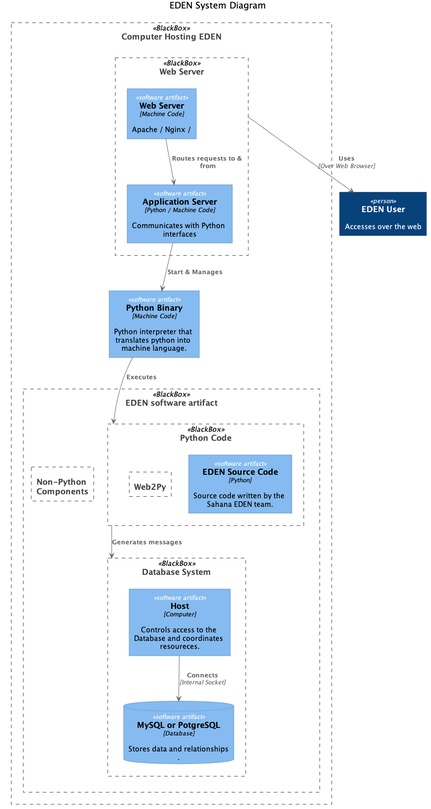
\includegraphics{images/EDEN_diagram.png}
   

   \subsection*{Why EDEN}
   I selected \acrshort{eden} for this project for two primary reasons: it is a \acrlong{foss} software project in a language I am familiar with and it is not obviously problematic. I will detail its open source pedigree shortly, but first I want to explain my second selection criteria. "Improving" software (whatever improving means) can usefully be separated into at least two questions: what quality should change and how do you bring that change about? This project attempts only to speak about the second (likely easier) question. Partially this is because the project was designed to fit within the confines of a final project for a masters degree. This project represents, roughly, three graduate level classes worth of work. I didn't feel like I had time to find \textit{and} fix flaws. So this project should be understood as neutral on the question of, "is \acrshort{eden} good?" Nothing about \acrshort{eden} seems bad to me. They have received numerous awards, glowing testimonials, and are used by many large organizations that could use other products if \acrshort{eden} were lacking. 

   I lack the experience and expertise to say that I think \acrshort{eden} is \textit{good}. Assessing if software is "good" or "bad" is not straightforward. Simply examining \glspl{sa} in isolation tell us very little. It's only through engaging with one or more \gls{sa}(s) as they exist in the lived world and contextualizing that with detailed ethnographic work that it's possible to start making value judgments \citep{Eubanks2018-hc,Schull2012-nc}. Those judgments wouldn't be universal, of course, but would be about a particular population. So this paper is done from the perspective that \acrshort{eden} seems fine to me. The project is interested in the technical details of how the \acrshort{eden} \gls{sa} emerges out of its \gls{sp} and how agency is modified by that process. 

   Finally, and briefly, this project does not take the position that the technical qualities it investigates are free from the impact of social structures. \citet{Gabriella_Coleman2012-lq} and \citet{Kelty2008-jm} have both compellingly shown that the social and technical co-produce each other. However, we can still usefully speak about qualities that technical systems have and how those qualities impact our lived experience. That this project has obvious extensions in the social and ethnographic realm is a strength and declining to investigate them should be understood as a concession to time.

   \subsection*{Out of Many, One}
   Wherever possible, \acrshort{eden} uses \acrshort{foss} technologies. The language it is written in, the libraries it relies on to provide functionality, the tools it uses to support its functionality, and its main operating system are all both open source and available at no cost. \acrshort{eden} will generally operate on top of non-\acrshort{foss} systems like Microsoft Windows, but the team doesn't prioritize systems outside of the \acrshort{foss} systems they develop and test on \citep{Sahana_Foundation2015-zs}. \citet{Kelty2008-jm} talks about how \acrshort{foss} is both a philosophy and a system of development that has practical impacts. One of the side effects of \acrshort{eden} committing to use the \acrshort{foss} ecosystem is it makes my form of engagement possible. Though it is possible to examine compiled machine code and draw some conclusions about the intent and process that assembled it, such a project would be far outside my capabilities. Instead, the source code of \acrshort{eden}, web2py (the \gls{web framework} \acrshort{eden} uses), Python (the language \acrshort{eden} and web2py are written in) and all of the libraries used by the project are open source. Their preferred databases (MySql or PostgreSQL) are also fully open source projects. Open source projects often don't just publish the current source code, but offer full histories of what change, when it changed, who changed it and how it was changed. These changes often include notes about why \textit{that particular} change was made over any other possible change \citep[p. 13-16]{Chacon2014-im}. Open source projects also commonly have systems for tracking lists of unfixed flaws as well as planned future improvements (both types of \citet{Mackenzie2006-hb} relationships), but those systems operate above the layer of source code so this project does not engage with them.

  \subsection*{Enumerating The Specifics of my Engagement}
  % much thanks to https://www.tablesgenerator.com/#
  \Acrshort{eden} has a large number of individual components. Executing a fully assembled \acrshort{eden} \gls{sa} would involve a number of \Gls{python} libraries, a number of other \glspl{sa} (a database, various compiled libraries) and a large amount of non-python code (such as the javascript contained in the \acrshort{eden} repository). Engaging all of this code is certainly possible if given enough time, but did not seem possible given the constraints of a masters project. So, I have chosen to focus on the \Gls{python} portions of a limit set of the libraries used by \acrshort{eden}. These libraries are listed in Table \ref{tab:table-1}\sepfootnote{libversions}. 

  \begin{table}[ht]
  \caption{Purpose of libraries}
  \label{tab:table-1}
  % https://stackoverflow.com/questions/2895780/how-to-code-tables-with-multi-line-cells
  \begin{tabular}{|l|p{.65\textwidth}|}
  \hline
  Component Name & Brief Description of Functionality                                                 \\ \hline
  Eden           & Implements the logic for managing the various resources Eden manages               \\ \hline
  web2py         & Provides interfaces to easily provide web services over HTTP and related protocols \\ \hline
  pydal          & Library for interacting with a database using Python objects instead of raw text   \\ \hline
  yatl           & Library for generating HTML content through templates                              \\ \hline
  \end{tabular}
% This MUST be at the start of the line without spaces before it or it will cause an error
% https://tex.stackexchange.com/questions/62278/problems-with-endfloat-package
\end{table}
  
  My choice to focus on these components in particular does not come from a considered opinion that these four components are the most important components. That judgement would require a good deal more work than I have done to develop an opinion about how to compare functionality across programming language boundaries. For the same reason, my analysis omits all non-programmatic components (databases, static content, etc). This omission should also be understood as a limitation imposed by time as opposed to a considered opinion that those components contribute less to the behavior of a \gls{sa}. 

  Instead, I chose these components because they were the ones I interacted with most during my investigation of the \acrshort{eden} project. There are also formal links between the projects: the \acrshort{eden} project identifies web2py as its \gls{webframework} and web2py identifies both pdal (as DAL) and yatl components of itself \citep{Di_Pierro2020-wn,Sahana_Foundation_undated-ww}. There are other primary components of the \acrshort{eden} project, but many of them are in other langauges or are themselves \glspl{sa} (such as databases).

  It's forseeable that my conclusions, focused on these four components, might not extend to the entire \gls{sa} / project, but I doubt it. In almost all circumstances, the components that most impacts what the \gls{sa} does would likely be in the \acrshort{eden} source code. That does not mean, as I will show, that most of the code that is associated with a particular element of an \acrshort{eden} \gls{sa} is within the \acrshort{eden} source code. It may be useful to refer to the size (in lines of code) of the various libraries to get a rough sense of the relative size of each one (See Table \ref{tab:table-2}). 

  \begin{table}[ht]
  \caption{Size of Libraries}
  \label{tab:table-2}
  \begin{tabular}{|l|c|c|}
  \hline
  Component Name & Lines of Python Code & Lines of Non-python Code \\ \hline
  Eden           & 469,117              & 793,661                  \\ \hline
  web2py         & 103,593              & 41,793                   \\ \hline
  pydal          & 24,518               & 416                      \\ \hline
  yatl           & 1131                 & 69                       \\ \hline
  \end{tabular}
\end{table}

  In general, the number of lines of code in a piece of software will correspond to that programs capabilities. Lines of code can also be used to roughly compare the relative contrabutions of components, especially when all components are written in the same language. It's possible to write lines of code that have no meaningful impact and it's easy to imagine scenarios where single lines of code make thousands meaningless (by turning off a feature, for insatance), but there is no reason to believe these instances would happen more or less often in any partcular component. Similarly -  it is much easier to imagine accomplishing the work done in fifteen lines of code with ten different lines, but it is much harder to imagine doing the work of fifteen hundred lines of code in a thousand. Efficient code is efficient, but there is a limit.



  \section*{Investigating EDEN}
   My work began, as all software work does, with work of assembling the components that transform \acrshort{eden} from a collection of \gls{python} source files into a \gls{sa}. This requires connecting a number of components together: libraries and tools in the gls{python} language and a wider set of heterogeneous tools (databases, non-\gls{python} libraries and tools). Some of these components remain as source code to be interpreted by \gls{python}, some of them are downloaded as source code and go through their own assembly process to generate their own \glspl{sa}. The assembly process that draws the components of \acrshort{eden} together does not happen in a single step, but is a number of loosely ordered heterogeneous processes. Some must be completed before others and there is an officially recommended order in which to prepare the various components, but often these orders are more matters of preference than necessity. What is important is that all of the required components are collected in their expected places by the time \acrshort{eden} itself is run. 

   The \gls{sf} recommends that developers use a \gls{vm} that has \acrshort{eden} and its supporting libraries installed through a script. However, at the time that I engaged with the project, the instructions for how to install \acrshort{eden} focused on using operating systems and \gls{python} versions that have since stopped being updated\sepfootnote{softwareupdates}. Though more modern scripts can be found, the standard install scripts for the \acrshort{eden} \gls{vm} and the script to install the software on a physical machine both use operating systems released in the mid-2010s that have not been maintained for at least 5 years \citep{Canonical2020-ru}. However, \acrshort{eden} is aware that this is problematic and makes an effort to support newer versions of \gls{python} and newer operating systems, but official instructions to use the latest software are sparse.

   \subsection*{Approaches to Tooling}
   Choosing to offer a fixed and unusually old set of tools is the first materialized I found encoded into \acrshort{eden}\sepfootnote{whatiseden}. The state of the scripts reflect a culturally important choice. The team could note and situate their approach in their documentation, but they have not. However, project-wise choices to use older or newer versions of tools are common. There are software projects (sometimes entire programming languages) that greatly value using the most up to date version of a tool or library \citep{Fernandes_da_Costa2017-mh}. These communities have legitimate fear that older versions of tools are examined less often and will likely be fixed less frequently. They feel that using the latest (within reason) version is a goodness in of itself\sepfootnote{releaselanguage}. If the \acrshort{eden} team followed this philosophy, they would not default to using older operating systems and versions of \gls{python}. They would need to watch their ecosystem of tools and libraries more closely, but the versions they were watching would also be more in the collective consciousness of the \acrshort{foss} world. 

   All this isn't to say that the \acrshort{eden} team choice isn't a sensible one. The latest versions of tools often lose track of the world outside the top of the capitalist pyramid. The same networks of power that structure the spread of physical technology also shape the attention of active software engineers. \acrshort{eden} has chosen to use established and well-supported versions of their tools\sepfootnote{stablecaveat}. Their older set of tools is more likely to have undiscovered (or unpatched) security vulnerabilities, but they are virtually certain to function properly and immediately allow the successful assembly of an \acrshort{eden} \gls{sa}. That set of probabilities seems very well suited to the expected audience for individuals first setting up their own copies of \acrshort{eden}: individual developers setting the system up to better understand it. When another team decides to deploy their own copy of \acrshort{eden} in a way that's available to the public, they can assemble that \gls{sa} using a balance of newness and stability that feels comfortable to them\sepfootnote{updaterisk}. 

   \subsection*{Investigating Assembly}
   It's one thing to identify where the \acrshort{eden} install scripts sit in a cultural gradient. It's another to engage the particular choices that the \acrshort{eden} project has made. I chose to install a far newer set of tools, based on the projects newest recommendations for new installs \citep{Konig2019-ya}. I was guided by the \gls{python} 2.7 installation script provided on the Sahana \acrshort{eden} wiki\sepfootnote{edensetup}. However, I chose to use a version of \gls{python} originally released in 2016 (six years after the default version used by \acrshort{eden}). Using a newer version of python seemed like a sensible software engineering choice and also a way to check if \acrshort{eden} was, as they claim, able to operate equally well on the version I selected (3.6.9) and the 2.7 version that \acrshort{eden} uses by default\sepfootnote{pythonversion}.

   Selecting a more modern \gls{python} turned out to have knock-on effects. Some of the libraries that \acrshort{eden} requires are written only for \gls{python} 2.7 and replacements were needed to function with 3.6. One of the major changes was that the version of \gls{w2p} the \acrshort{eden} scripts installs does not support \gls{python} 3.6 and so I needed to chose an updated version. I selected 2.18.5, but this new combination of the \acrshort{eden} source code and the \gls{w2p} source code revealed that the two projects had drifted apart in small but essential ways. Specifically, in a section of the \gls{w2p} and \acrshort{eden} code that handled data validation.

   Data validation is, in general, the work of verifying that information conforms to a set of standards and informing the user how it has failed to conform when a problem is found. This should always be performed any time data is stored in a system. Digital storage systems have expectations that, when violated, can cause immediate systems failures. Web frameworks commonly provide facilities for verifying data and \gls{w2p} is no exception. \Gls{w2p} has components that will check that that user input can be converted to numbers or dates or email addresses, among others. \Gls{w2p} is open source and so all of that functionality can be expanded by programs that make use of \gls{w2p} and \acrshort{eden} does so in a number of places.

   \subsection*{Shifting Relationships}
   In between the version of \gls{w2p} that \acrshort{eden} uses by default and the version of \gls{w2p} that I selected, the control flow of data validation has changed slightly. This change meant that custom data validation classes that were written using the older \gls{w2p} system no longer fit into the expected control flow of data validation. The \acrshort{eden} data validation code, based on the older standard, is not called properly when using the newer version of \gls{w2p}. This doesn't stop the successful assembly of an \acrshort{eden} \gls{sa}, but once that \gls{sa} is assembled most of its functionality in inaccessible because the \acrshort{eden}-specific data validation code won't run and so the system won't accept that data. 

   This problem is interesting because it turns out it captures a moment in time between the \gls{w2p} team and the teams that use \gls{w2p} (i.e. \acrshort{eden}). If I had selected a slightly earlier version of \gls{w2p}, then it would have used the old system and the \acrshort{eden} code would remain functional. \gls{w2p} immediately realized the problem and integrated a fix\sepfootnote{problemfix} for the issue. This shows the management of relationships that \citet{Mackenzie2006-hb} describes. There is the work of making software and then the subsequent and parallel work of adjusting that software to stay within relationships boundaries. The \gls{w2p} successfully implemented a new way of handling data validation control flow, but they neglected that they were doing it in such a way as to break an existing relationship they did not mean to break. Because I happened to select a version of \gls{w2p} that was temporarily out of relation with \acrshort{eden}, I failed to assemble a fully functional \gls{sa}. This was what got me interested in the assembly process itself.

   \subsection*{Investigating Assembly}
   Assembly is a label I'm using to cover a variety of software processes that source code (and many other things) and produce \glspl{sa}. Almost all software is written in programming languages that have the dual goal of being possible for humans to understand and being suitable for mechanical translation into machine code. Machine code is, after all, the only language a computer can really understand \citep{Cramer2008-cw}. 

   Methods of assembly vary widely, but they can roughly said to lie between compilation and interpretation. The purest compiled language will generate a \gls{sa} that contains all the machine code that will be used by the \gls{sa} into a single contiguous piece of machine code. That machine code will generally only work on a single hardware architecture, but the same source code can be assembled\sepfootnote{compilelanguage} into machine code on other architectures by different assembly tool-chains. On the other side of this spectrum are interpreted languages. A purely interpreted language assembly process does not involve the generation of any new machine code. Instead, it uses a standard \gls{sa} (called an "interpreter") that reads the source code of the interpreted program in its human readable form like a recipe: reading the file(s) as the interpreted program executes and using machine code that exists within the artifact of the interpreter to tell the hardware what to do.

   There are also a variety of methods for \glspl{sa} to share access to centers of functionality. The most common is sending calls "out" to libraries. The pure compilation situation described above really only exists on hardware without a multitasking operating system. For every \gls{sa} on your phone or computer, the \gls{sa} will frequently make a call to a library (which itself sits somewhere between compiled and interpreted) where it specifies which library, which section of the library, and the information it would like to pass off. Then the operating system pauses the execution of the machine code in the \gls{sa} and loads the library (or the library's interpreter) to perform the requested task. When the task is done, the first \gls{sa} is loaded again and told the result. 

   Most languages and \glspl{sa} sit somewhere between being fully compiled and fully interpreted. \Gls{python} is largely an interpreted language, but it also creates non-human readable bytecode versions of each python source file that allow the interpreter to execute more quickly \citep{The_Python_Software_Foundation2020-qz}. \Gls{python} also allows access to libraries written in machine code and \acrshort{eden} invokes machine code libraries through \gls{python} interfaces.

   \subsection*{Digital Relationships}
   These libraries exist on the border of all of the \glspl{sa} that use them\sepfootnote{staticlink}. They contribute to how the \glspl{sa} that use them behave. Flaws in libraries can allow the programs that use them to be taken over. Sometimes these flaws only require attention to discover, but it's often the case that other elements of the hardware / software ecosystem must change before they can be found \citep{Huang2003-ki}. All this is to say that the kind of assembly problem I encountered in assembling \acrshort{eden} is not particular to \acrshort{eden}. It's a universal concern when assembling \glspl{sa} that use any functionality that resides outside their own source code (which nearly all do).

   This system of linking together different code written by different people is an example of the relationships that \citet{Mackenzie2006-hb} found at the center of the software projects he studied. At the project level this means that a the people working on one project must pay attention to the development of many other projects. Are new versions of the libraries that you use being released? Will the old version be updated if security flaws are found? Does the new version have features or changes that would be useful for our project? 

   What is striking about the problems encountered while trying to assemble my own artifact of \acrshort{eden} is that, while every individual who assembles an \acrshort{eden} \gls{sa} will need to go through their own process, the problems I encountered are particular to using an un-patched version of \gls{w2p} 2.18.5. The install script I used contains other fixes for other aspects of that particular pairing of components, as well as different fixes for different combinations of components \citep{Sahana_Foundation2018-eq}. \acrshort{eden} can be assembled using an extremely wide set of components. It can run on that haven't been considered up to date for over ten years ago and components that are still considered cutting edge now (as well as many mixes between these two extremes). The \acrshort{eden} \gls{sa} is designed with this capability in mind. It is a strength of the \acrshort{foss} ecosystem that such a wide range of compositions is possible, but it also means that \acrshort{eden} can be a nearly limitless number of different \glspl{sa} whose qualities emerge both from \acrshort{eden}'s source code and the interactions between the particular versions of the components.

   \subsection*{The Social and Material Components of Software}
   Keeping in mind the range of possible component sets for \acrshort{eden}, think back to the particular set used in the install script. I speculated the set in that script were selected because they're well known familiar to the \acrshort{eden} development team. They minimize the chance that people will mistake a problem caused by assembly for a problem that exists within the \acrshort{eden} source code.  

   When a particular \gls{sa} fails to function as expected, there are many possibilities as to why. It might be mis-configured, the resources it needs to function properly might not be available, there may be an internal incompatibility between components, or there may be an error in the \acrshort{eden} source code. There are many functional \acrshort{eden} \glspl{sa} that contain component combinations that the developers have never tried and have no experience with. When what appears to be an error is reported to the \acrshort{eden} team, often the first questions they ask are about the versions of the libraries that were involved. If the versions of the libraries being used aren't considered to be the correct ones, the bug can be closed as wholly or partially invalid \citep{Trendspotter2020-ps}.

   This method of engagement around questions of proper assembly and proper component selection are, above all, practical. Over time the number of possible combinations of all the versions of all the libraries will inevitably expand beyond the abilities of any team. To control this somewhat, teams will have defined periods of support and lists of appropriate versions of components and only fix problems that found within that somewhat limited domain \citep{Canonical2020-ru,Konig2019-ya}. But \glspl{sa} that are assembled using components drawn from outside the official set of components may still function. Being 'out of support' does not mean that things will not work. It means that the team managing the software project has no opinion about the relationships between their code and the components you're using. They will support the official supported combinations and leave you to do your best with the unofficial ones.

   This suggests a limit on the boundaries of the \acrshort{eden} software project. Maybe the unofficial \glspl{sa} that the \acrshort{eden} team won't support now aren't really \acrshort{eden} \glspl{sa}. However, I don't think it's that simple. What components (and versions of the \acrshort{eden} source code itself) are inside the 'official' \acrshort{eden} change over time. What is an unofficial \acrshort{eden} \gls{sa} might one day become an official software version as the \acrshort{eden} software project changes its thinking about relationships. By the same stroke, official versions will often become unofficial. The team recently announced that, with the end of official support for \gls{python} 2, they will be moving to using \gls{python} 3 for all of their builds and updating their install scripts to use \gls{python} 3. Suddenly, my \acrshort{eden} \gls{sa}, which already uses \gls{python} 3 is within the official definition and the \acrshort{eden} \gls{sa} assembled by the script on the Sahana website is unofficial \citep{Konig2019-ya,Sahana_Foundation2015-zs}. 

   \subsection*{Software Exists Outside of the Social}
   Instead, I think what this shows is a material reality interacting with a social relationship. Each given version of \acrshort{eden}'s source code has a particular material relationship with each version of each component it could use. These relationships have an existence outside of any social system because computer code can be executed mechanistically \citep{Cox2013-zo}. The official / unofficial layer, where the team that writes the source code for \acrshort{eden} and sets forth the list of officially supported component relationships, exists on top of this material reality. But this social layer does not change what software \textit{is}.

   Understandings of software where only the official versions of \acrshort{eden} are "the software called \acrshort{eden}" lead to an understanding of software that defies common experience. It would mean that, once the \acrshort{eden} team announced that they were migrating away from \gls{python} 2, all of the \gls{python} 2 \acrshort{eden} \glspl{sa} that exist and function now suddenly stopped being software. It would also mean that, because I have changed some elements within the \acrshort{eden} source code\sepfootnote{sourcemodifications}, my \gls{sa} can no longer be \acrshort{eden} - even if I used all the official supporting components. It would require an impossible level of information about every component and every element of every \gls{sa} that appears to be \acrshort{eden}.

   Once we accept both official and unofficial \glspl{sa} are that software, it becomes clear that another social understanding exists along side just the official and unofficial version of software. Most people who encounter a particular software project have no idea if they are interacting with an official or unofficial version\sepfootnote{unofficialbinaries} (or that such a distinction even exists). So there exists this general social understanding about each piece of software (including \acrshort{eden}) that individual draw from their own experiences. These experiences might be with official software, unofficial software, or even be based on a mis-identification of the software (such as receiving a counterfeit product and leaving a bad review for the original) \citep{Suthivarakom2020-cp}.

   It's useful to draw out these different social experiences of software because it allows us to think in a more informed way about the impact of materialized perspectives. It is not just the source code of a particular software project that adds to its behavior, it is also the various components that source code is combined with. For those who only interact with post-assembly \glspl{sa}, the relationship of the software they are using to the official software is unknowable. Software that has the reputation for being unstable and unreliable can get that reputation because people are, knowingly or unknowingly, using pirated copies that crash because of anti-piracy code \citep{Fitch2008-vq}. The team that makes that piece of software may never know why people think its unstable, because they would need to understand the assembly processes that particular \glspl{sa} went through. The users may want the software to be different, but though the software team is the single entity most responsible for how a particular \gls{sa} functions, they may simultaneously be unable to understand or repair the problem.


   \subsection*{Reckoning with Failures}
   After assembling a functional \gls{sa} I began to explore how my \acrshort{eden} \gls{sa} functions on its own terms. I did this by entering the high level details of this project into \acrshort{eden}'s project tracking feature. This included creating an entry for Drexel University's Center for Science, Technology and Society, an entry for my project within that organization, and an entry for myself as the manager of that project. During this process I encountered both a bug in the source code of \acrshort{eden} and another unacknowledged materialized perspective. 

   The form that \acrshort{eden} uses to record the details of an individual has a field for a phone number. There's no indication that this number number should be formatted in one particular way over another. I didn't think anything the lack of instruction until my \acrshort{eden} \gls{sa} informed me that I needed to "Enter a valid phone number" \citep{Konig2020-yx}. I didn't understand because my phone number was following the common conventions for phone number formats (I tried the 'xxx.xxx.xxxx' as well as 'xxx-xxx-xxxx' and 'xxxxxxxxxx'). Upon review of the source code of the file responsible for the message I discovered two things: that, based on a setting I was not aware of, the form was expected a phone number in international format (beginning with a '+' and a country code) and that the code was returning the wrong message (complaining that the input was not a phone number instead of complaining it was not an international phone number). After entering my number in the international format, my profile was created.

   % maybe conclusions
   This felt like an excellent situation to investigate. It appears, on first brush, that there are two layers of unacknowledged materialized perspectives: the first being requiring numbers to be in the international format without informing the user filling out the form, the second appears to be an error in the message returned. My background as a programmer and my access to the source code makes me want to say that the \acrshort{eden} project intends to require international numbers and failed to return the correct message about that requirement. However, I think it is worth considering how these two problems appear without access to the source code.

   First - imagine if the second problem was fixed (the \gls{sa} returned the proper error). When the user enters a number without a country code, the \acrshort{eden} \gls{sa} will reject their number and tell them it must be international. They now know what to do, but had no way to learn about the requirement before they failed to meet it.

   Second - imagine if the \gls{sa} informed the user they needed to enter their number with an international country code. But, when the code was left off, told the user their number wasn't valid. Again, the user would not be sure what to do to advance. It might be easier to find out (because the \gls{sa} has labeled the field with the requirement), but \textit{from the users' point of view} these two situations are very similar. It is only the ability to look into the source code that clearly sets them apart.

   % findings
   So, after discovering it, I decided to see what I could learn by giving back to the \acrshort{eden} project and fixing this (extremely minor) bug. I wrote and submitted a small patch that intended to fix the problem and check that the proper error message was returned. Unfortunately, much to my embarrassment, my fix was written incorrectly - it incorrectly eliminated another error message that could, in certain circumstances, be displayed to the user. As a result my fix was rejected, though once the \acrshort{eden} project was aware of the bug they immediately wrote their own fix \citep{Konig2020-ey}.

   In the discussion about why my fix was flawed, one of the \acrshort{eden} project developers said several interesting things about how he (and by extension the \acrshort{eden} project) think about software.

   \begin{quote}
   "And no, there's no test case as to what error message exactly is returned.

   Whilst we could unit-test it routinely, \textbf{regression-testing too much detail can add excessive rigor thus make development harder}. \textbf{A wrong error message is an annoyance, but neither does it break the intended functionality}, nor does it jeopardize the data integrity - so it is low priority and should probably not be CI-tested." \citep{Konig2020-yx}\sepfootnote{longquote}
   \end{quote}

   There are a couple of interesting ideas in this quote that, I think, can help us understand how software (or at least the \acrshort{eden} project) functions. First, there's the idea that testing too much makes development harder. Since K{\"o}nig is talking about regression testing (testing of fixed bugs) the difficulty would likely come from tests unexpectedly failing after changing related code or would come from work needed to update the test when changing the functionality it is testing\sepfootnote{ethnographylimits}. In any case, the decision to limit testing is also a decision to limit their automated testing to a certain subset of all program functionality. That development would be harder if the full scope of possible functionality was tested and that it is better to be ignorant about ancillary behavior like error messages.

   The second idea is that accepting or rejecting the number based on its use of an international country code (which it does successfully) and informing the user of what they need to do should be considered separately. That however the program appears to to the user, if it accepts numbers in the desired format and rejects others then the component is working. The statement reflects a world view that, if a component is expected to have multiple outputs for a given input, each output should be considered working or non-working separately and that there is a hierarchy to which functions are more or less important. 

   % discussion
   \subsection*{Implications of my failed bug fix}
   Before going into the interesting aspects of the K{\"o}nig quote, I want to talk about something I find interesting about the context of how the discussion about the bug took place. This was, as I said, a discussion between people who both had access to one (or more) \acrshort{eden} \glspl{sa}. I originally noticed the bug when I was interacting with my \gls{sa}. This is in line with how most software projects come to have an impact on the world: through directly or indirectly affecting the world through the \glspl{sa} that the project produces or makes possible \citep{Kitchin2011-af}. While software impacts our lives in direct and indirect ways, those impacts derive from how one or many \gls{sa}(s) interact with particular human agents. Though software has made is possible to remove humans at many of the intersections of power, it is still expressed through a multitude of relational contacts between a representative of power (a person or a \gls{sa}) and a human outside that power \citet{Cheney-Lippold2018-lw,Deluze1995-eo}. 

   \subsection*{Do Software Artifacts Matter}
   Given all of that, I think it's interesting to note that the entire discussion about bugs took place without referencing the behavior of any particular \gls{sa}. I've already speculated that the \acrshort{eden} project may recommend older components to minimize the risks of improper assembly and that questions \textit{about} the correctness of assembly are common \citep{Trendspotter2020-ps}. Because investigating the particulars of a misbehaving \gls{sa} are common, the lack of discussion here is interesting. 

   When a \gls{sa} is under discussion, that discussion often proceeds with the implicit goal of finding a mistake or a mismatched relationship in the assembly process. My bug fix, in contrast, was to a particular pre-assembly component. In order to realize my change, a new \gls{sa} would need to be assembled. Nothing in my attempt to fix the bug or in the eventual official bug fix can repair existing \glspl{sa} \citep{Konig2020-yx,Konig2020-ey}. This explains the lack of interest in any existing \gls{sa} - nothing about any \gls{sa} that might or might not express this bug is of interest. Instead, when the bug is fixed in a component of \acrshort{eden}, any potentially problematic \gls{sa} will be replaced with a new one assembled from updated components.

   % https://stackoverflow.com/questions/1945075/how-do-i-create-binary-patches
   To underline this point again - \glspl{sa} are never updated. When a 'patch' is applied to a \gls{sa}, the goal of that patch is to make the existing \gls{sa} identical to the \gls{sa} that would be generated by a fresh assembly. This means that a patch program is a new \gls{sa} that will effectuate a different assembly process than usual with the goal of producing the same outcome as a full re-assembly with all components \citep{Endsley_undated-iy}. It's also common for a \gls{sa} to contain many internal \glspl{sa} and for a patch to replace one or more component \glspl{sa} in full. However, the \glspl{sa} that accomplish these tasks of updating existing \glspl{sa} are separate \glspl{sa} in their own right. A software project can choose to utilize them or not utilize them, but their choice won't change how they "fix" problems found in an existing \gls{sa}. 

   The bug was fixed by changing a component with the intent of that component being assembled into a new \gls{sa}. It could also have been repaired by creating a new \gls{sa} to intentionally make changes to existing \acrshort{eden} \glspl{sa}, but this would need to be repeated for every previous \gls{sa}\sepfootnote{interpreted}. So \glspl{sa} are always replaced, because digital technology makes it easy to do so and the practical consequences are the same either way: a particular number of bytes in a particular order on digital storage. 

   This means that scholars must be careful when applying concepts whose identities were formed based on our collective experiences with physical goods. It's true that software is maintained, updated, repaired, cleaned, polished, and so on. Those operations often serve the same purpose as similar operations on physical tools, but the material character of how they are carried out will be dramatically different. This will impact the worlds of the people doing the work, the particulars of how these operations change the operation of software, and the proper weighting of concerns in assessing the impact of these operations. Because the material that composes the physical character of \glspl{sa} is cheap and plentiful (electrical charge), many of the previous systems that evolved in response to more complicated systems of material construction have limited implications for software projects and \glspl{sa}.

   \subsection*{The Limits of Developer Attention}
   I want to briefly expand on the idea, expressed by K{\"o}nig, that testing in too much detail can harm software development. I think this idea, in combination with some discussion of assembly in the following section, will be helpful for thinking about agency in software. An uncharitable understanding of the idea that too much testing harms development is that developers might not care about some dysfunction, but I see no evidence of this. The \acrshort{eden} project immediately implemented a fix for the problem I found, even though they do not wish to add a test for it. 

   Instead, I think this approach reflects a \citet{Citton2017-xq}-esq approach to the problem posed by the enormous complexity of \glspl{sa}. In just the 4 libraries

   % todo: finish

   \subsection*{What does Working Mean Here?}
   I want to return to talking about the various experiences of functionality and non-functionality I've encountered in this work \sepfootnote{working}. First I'm going to try and explore the ideas of assembly and then how to think about the functionality of assembled artifacts.

   Assembly is a process whose limits are challenging to clearly mark. There are instances where assembly is clearly successful, such as when a \gls{sa} works correctly in all ways or in instances where the failure of an assembled \gls{sa} clearly comes directly from a single flaw in a single component (such as the international number bug). There are also limits where assembly is clearly unsuccessful: when a component cannot be found, when a language that must be translated into machine code (or any language) is found to contain a syntax error \citep{Cramer2008-cw}. However, when I created a software artifact that failed to work because of a broken relationship between its components, I began to wonder if my definition of assembly was flawed.

   Unlike compiled languages, which fully parse their constituent source files before reaching a state where an executable \gls{sa} exists, Python \gls{sa} performs assembly immediately before executing a python program\sepfootnote{runtimeimports}. In fact, the \gls{python} assembly is piecemeal - each file is only read when needed, so files that are part of the \gls{sa} could go unused for any period of time before being used in the \gls{sa}. It would be possible to, for instance, begin running an \acrshort{eden} \gls{sa} and replace the line of web2py code that, if it were executed, would cause a crash. If the code was replaced before the \acrshort{eden} \gls{sa} called the code with the bug, no crash would occur. So do I need one approach for assembly with interpreted languages and another approach with compiled languages?

   No, because the apparent differences are illusions. Compiled programs can also have their contents changed mid-executions (this is the usual method for 'breaking into' a computer). Changing the contents of a program that has already been translated to machine code is simply much less convenient than changing the text in the source file of an interpreted language. The moment of failure that I encountered when web2py tried to invoke \acrshort{eden} code it no longer knew how to find was a moment where the computer tried to follow a chain of relationships. It would not be possible to know if any given instance of an \acrshort{eden} validator that inherits from web2py code would work correctly without running the program. This means that finding the error would require solving the halting problem, which is impossible \citep{Kaplan_undated-xy}. 

   For the purposes of this this project, what I call assembly is every aspect of preparing a program to execute that can be done without needing to actually execute the program (i.e. the limits of the halting problem). These processes (compilation, the locating of python files) are often themselves executed by \glspl{sa}. As long as the work being done could be done without executing source code, it is considered part of the assembly step\sepfootnote{pythonexeq}. 

   Why is this important? Does it matter for sociologists when assembly stops and execution begins? The end of assembly is the point where human intervention into a \gls{sa} largely stops being useful. After assembly is complete, the balance of which components will impact the overall behavior of the \gls{sa} is fixed. The only human intervention that is possible is the decision to start or stop the \gls{sa}\sepfootnote{askingforhumaninput}. This is doubly important because our ability to predict what a \gls{sa} will do when it is executed is hampered by both practical and theoretical limits \citep{Kaplan_undated-xy}. 

   This reality is reflected the practice of testing in the development of \glspl{sa}. The \acrshort{eden} \gls{sa} assembled in \acrshort{eden}'s test code is not exactly like the final \gls{sa} (it largely differs in the database entries that compose it), but the goal is to make it as close as possible to the final \gls{sa}. For instance, the assembly error I encountered with web2py was easily detected by tests. Testing is a reaction to the fixing of agency in a \gls{sa} and an attempt to ensure that the agency reflected in the final \gls{sa} is sufficiently similar to the developers' intent. These tests can take the form of source code that is incorporated into one or more testings \glspl{sa} or in planned interaction with the final \gls{sa} before releasing it to the public. 

    
    \printnoidxglossaries

   \section*{Long Tables}
   These tables are missing some information that is available in this google sheet: \url{https://docs.google.com/spreadsheets/d/1fi5cNCA1mQgS8gZ7VL7MfalSXNQoD2pM1vC3uH18cNw/edit}. Additionally, the contributor who is identified as 'sherdim' used their real name, but I was unable to get \LaTeX to display their name properly, so I have used their github handle. Their profile can be found here: \url{https://github.com/sherdim}.

\begin{table}[ht]
\caption{Eden Contributors}
\label{tab:contribs-1}
\begin{tabular}{|l|r|r|}
\hline
Name            & Related Changes & Total Changes \\ \hline
Ashwyn          & 69              & 7,580         \\ \hline
Aviral Dasgupta & 88              & 6,147         \\ \hline
biplovbhandari  & 18              & 2,6692        \\ \hline
Daniel Drexler  & 69              & 10,342        \\ \hline
Dominic König   & 33,934          & 1,940,890     \\ \hline
Fran Boon       & 23,604          & 3,816,361     \\ \hline
Graeme Foster   & 646             & 241,090       \\ \hline
hitesh96db      & 8               & 13,588        \\ \hline
James O'Neill   & 4               & 4,038         \\ \hline
Kunal Hari      & 33              & 8,920         \\ \hline
Michael Howden  & 755             & 143,771       \\ \hline
Pratyush Nigam  & 312             & 290           \\ \hline
raj454raj       & 1               & 10,917        \\ \hline
redsin          & 810             & 25,265        \\ \hline
tirgil          & 2               & 3,804         \\ \hline
VishrutMehta    & 6               & 1,153         \\ \hline
\end{tabular}
\end{table} 

\begin{table}[ht]
\caption{pydal Contributors 1}
\label{tab:contribs-2.1}
\begin{tabular}{|l|r|r|}
\hline
Name                 & Related Changes & Total Changes \\ \hline
abastardi            & 189             & 15            \\ \hline
alan                 & 8               & 11            \\ \hline
boa-py               & 4               & 2             \\ \hline
BuhtigithuB          & 9,035           & 5,524         \\ \hline
Cássio Botaro        & 2               & 2             \\ \hline
Christophe Varoqui   & 42              & 2             \\ \hline
Dan Feeney           & 11              & 11            \\ \hline
David Orme           & 160             & 30            \\ \hline
Dominic König        & 15              & 43            \\ \hline
dz0                  & 12              & 1             \\ \hline
Emmanuel Goh         & 68              & 4             \\ \hline
Fran Boon            & 75              & 21            \\ \hline
Francisco Tomé Costa & 8               & 4             \\ \hline
gi0baro              & 75,295          & 69,785        \\ \hline
Giovanni Barillari   & 17,667          & 8,240         \\ \hline
ilvalle              & 16,027          & 37,158        \\ \hline
Jack Kuan            & 147             & 7             \\ \hline
JusticeN             & 15              & 15            \\ \hline
jvanbraekel          & 381             & 40            \\ \hline
kvanzuijlen          & 116             & 2             \\ \hline
Leonel Câmara        & 1667            & 896           \\ \hline
Name                 & Related Changes & Total Changes \\ \hline
\end{tabular}
\end{table}

\begin{table}[ht]
\caption{pydal Contributors 2}
\label{tab:contribs-2.2}
\begin{tabular}{|l|r|r|}
\hline
Name                 & Related Changes & Total Changes \\ \hline
Martin Doucha        & 9,233           & 3,037         \\ \hline
maxcrystal           & 11              & 11            \\ \hline
Massimo DiPierro     & 22,447          & 903,691       \\ \hline
Michael Loster       & 4               & 2             \\ \hline
Michele Comitini     & 541             & 5,975         \\ \hline
nikakis              & 216             & 18            \\ \hline
niphlod              & 5,178           & 30,396        \\ \hline
preactive            & 2               & 2             \\ \hline
Remco Boerma         & 20              & 5             \\ \hline
Richard Boß          & 5               & 5             \\ \hline
rodwatkins           & 56              & 14            \\ \hline
Stephen Rauch        & 6,166           & 4,993         \\ \hline
Stephen Tanner       & 11              & 43            \\ \hline
Tim Nyborg           & 82              & 6             \\ \hline
Tom Stratton         & 36              & 9             \\ \hline
Victor Salgado       & 44              & 18            \\ \hline
Vinyl Darkscratch    & 24              & 49            \\ \hline
Wanderson Reis       & 53              & 5             \\ \hline
willimoa             & 7               & 64            \\ \hline
xuyangbocn           & 24              & 2             \\ \hline
Christophe Varoqui   & 2               & 2             \\ \hline
dz0                  & 1               & 1             \\ \hline
\end{tabular}
\end{table}

\begin{table}[ht]
\caption{yatl Contributors}
\label{tab:contribs-4}
\begin{tabular}{|l|r|r|}
\hline
Name                           & Related Changes & Total Changes \\ \hline
Carlos Cesar Caballero Díaz    & 17              & 17            \\ \hline
Massimo DiPierro               & 2,312           & 2,089         \\ \hline
PhanterJR                      & 254             & 263           \\ \hline
\end{tabular}
\end{table}

\begin{table}[ht]
\caption{web2py Contributors 1}
\label{tab:contribs-3-1}
\begin{tabular}{|l|r|r|}
\hline
Name                           & Related Changes & Total Changes \\ \hline
abastardi                      & 37              & 153           \\ \hline
Adam Bryzak                    & 2               & 2             \\ \hline
Alexander Zayats               & 16              & 8             \\ \hline
alexdba                        & 34              & 17            \\ \hline
Alfonso de la Guarda Reyes     & 27              & 63            \\ \hline
Anssi Hannula                  & 20              & 12            \\ \hline
Batchu Venkat Vishal           & 2               & 2             \\ \hline
Carlos Cesar Caballero Díaz    & 68              & 3,136         \\ \hline
Carlos Costa                   & 26              & 236           \\ \hline
Cássio Botaro                  & 22              & 207           \\ \hline
cccaballero                    & 10              & 138           \\ \hline
Chen Rotem Levy                & 8               & 309           \\ \hline
Chris DeGroot                  & 8               & 4             \\ \hline
Chris Garcia                   & 12              & 34            \\ \hline
clach04                        & 90              & 45            \\ \hline
Daniel Libonati                & 4               & 9             \\ \hline
Denis Rykov                    & 8               & 4             \\ \hline
Dinis                          & 4               & 470           \\ \hline
Dominic König                  & 4               & 10            \\ \hline
Donald McClymont               & 7               & 7             \\ \hline
Erik Montes                    & 4               & 147           \\ \hline
Fran Boon                      & 20              & 28            \\ \hline
geomapdev                      & 306             & 223           \\ \hline
gi0baro                        & 29,055          & 38,807        \\ \hline
Giovanni Barillari             & 105             & 346           \\ \hline
hectord                        & 6               & 6             \\ \hline
ilvalle                        & 3,857           & 65,421        \\ \hline
Jack Kuan                      & 16              & 24            \\ \hline
Jan Beilicke                   & 26              & 13            \\ \hline
Jan M. Knaup                   & 24              & 12            \\ \hline
Jaripekkaf                     & 112             & 56            \\ \hline
Jeremie Dokime                 & 18              & 54            \\ \hline
Joel Rathgaber                 & 22              & 22            \\ \hline
Jonathan Bohren                & 59              & 59            \\ \hline
Jonathan Vasek                 & 4               & 2             \\ \hline
Jose C                         & 2               & 1             \\ \hline
jvanbraekel                    & 124             & 108           \\ \hline
kelson                         & 40              & 306           \\ \hline
Kiran Subbaraman               & 98              & 99            \\ \hline
Koen van Zuijlen               & 4               & 8             \\ \hline
Kristján Valur Jónsson         & 2               & 2             \\ \hline
\end{tabular}
\end{table}

\begin{table}[ht]
\caption{web2py Contributors 2}
\label{tab:contribs-3-2}
\begin{tabular}{|l|r|r|}
\hline
Name                           & Related Changes & Total Changes \\ \hline
Kurt Grutzmacher               & 352             & 2,378         \\ \hline
Leonel Câmara                  & 1,444           & 14,051        \\ \hline
Lisandro                       & 8               & 14            \\ \hline
Luca de Alfaro                 & 2               & 2             \\ \hline
Martin Doucha                  & 92              & 99            \\ \hline
Massimo DiPierro               & 146,548         & 825,014       \\ \hline
Mathieu Clabaut                & 48              & 88            \\ \hline
mcabo                          & 56              & 28            \\ \hline
Michele Comitini               & 2215            & 6034          \\ \hline
mictee                         & 33              & 71            \\ \hline
Mirko Galimberti               & 22              & 52            \\ \hline
mpranjic                       & 12              & 36            \\ \hline
Nik Klever                     & 10              & 45            \\ \hline
niphlod                        & 10,189          & 45,996        \\ \hline
Oleg                           & 82              & 43            \\ \hline
Omar Trinidad Gutiérrez Méndez & 14              & 321           \\ \hline
omniavx                        & 4               & 2             \\ \hline
Oscar Fonts                    & 32              & 585           \\ \hline
Oscar Rodriguez                & 132             & 66            \\ \hline
Paolo Caruccio                 & 12              & 475           \\ \hline
Prasad Muley                   & 46              & 23            \\ \hline
Radu Ioan Fericean             & 30              & 66            \\ \hline
Ricardo Pedroso                & 216             & 263           \\ \hline
Richard Vézina                 & 9,605           & 17,379        \\ \hline
samuel bonilla                 & 4               & 93            \\ \hline
Scimonster                     & 4               & 6             \\ \hline
Seth Kinast                    & 10              & 18            \\ \hline
spametki                       & 946             & 3,404         \\ \hline
Stefan Pochmann                & 120             & 114           \\ \hline
tiago.bar                      & 2               & 4             \\ \hline
tim                            & 4               & 2             \\ \hline
Tim Nyborg                     & 84              & 109           \\ \hline
Tim Richardson                 & 444             & 337           \\ \hline
viniciusban                    & 34              & 261           \\ \hline
Vinyl Darkscratch              & 410             & 121,159       \\ \hline
winniehell                     & 5               & 5             \\ \hline
zvolsky                        & 22              & 1,543         \\ \hline
sherdim                        & 2               & 14            \\ \hline
Luca de Alfaro                 & 2               & 2             \\ \hline
Jonathan Vasek                 & 2               & 2             \\ \hline
Jose C                         & 1               & 1             \\ \hline
\end{tabular}
\end{table}
   \setlength{\parindent}{4em}
   \bibliography{Final_Draft}

\end{document}